%
%
%		Finding: Template
%		Author: the DR
%
%
\renewcommand{\FindingAuthor}{Michal Olencin}
% DO NOT USE \par, \newline or any other line breaking command in FindingName => report will not build
\renewcommand{\FindingName}{Sensitive Information Disclosure via Logging}
\renewcommand{\Location}{dummyapplication.apk, dummyapplication.ipa}
\renewcommand{\Component}{Logcat}
\renewcommand{\FoundWith}{Manual testing}
\renewcommand{\TestMethod}{Manual}
\renewcommand{\CVSS}{4.0}
\renewcommand{\CVSSvector}{CVSS:3.1/AV:L/AC:L/PR:N/UI:N/S:U/C:L/I:N/A:N}
\renewcommand{\CWE}{532}
% Poor-man's combo boxes:
% High, Medium, Low, Info, TBR (To Be Rated)
\renewcommand{\Criticality}{Medium}
% Easy, Average, Hard, TBR (To Be Rated)
\renewcommand{\Exploitability}{Easy}
% Access control, Application Design, Information Disclosure, Outdated Software, Security Configuration
\renewcommand{\Category}{Undefined}
% Easy, Average, Difficult, TBR (To Be Rated)
\renewcommand{\Detectability}{Easy}


\ReportFindingHeader{\FindingName}


%-------------------------------------------
%	Details                                |
%-------------------------------------------

\subsection*{Details}

Sensitive information like JWT and exception stacktrace is being written to the logs, making it accessible to unauthorized parties.


%-<Details>
%-------------------------------------------
%	Impact                                 |
%-------------------------------------------



\subsection*{Impact}

The presence of sensitive information in the console creates a security risk as attackers could potentially access and misuse the information, leading to data breaches and other negative consequences.

%-<Impact>
%-------------------------------------------
%	Repeatability                          |
%-------------------------------------------



\subsection*{Repeatability}

During the static analysis it was observed, that the value of the cache (including JWT) is logged at level \texttt{info} in the method \texttt{saveString} (see \cref{figure:code_jwt}).
Additionally, observe that the exception stack trace is logged at level \texttt{error} in the method \texttt{saveString} (see \cref{figure:code_exception}).
In \cref{figure:code_enabled} is snippet that sets the log level.
Since the level is set to \texttt{info}, both JWT  and exception stacktrace are logged.

\begin{figure}[H]
\centering
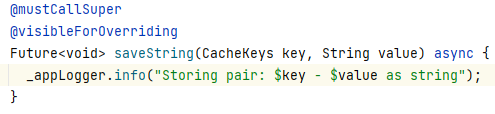
\includegraphics[width=0.8\textwidth,frame]{\CurrentFilePath/code_jwt.png}
\caption{Snippet of the \texttt{saveString} method}
\label{figure:code_jwt}
\end{figure}

\begin{figure}[H]
\centering
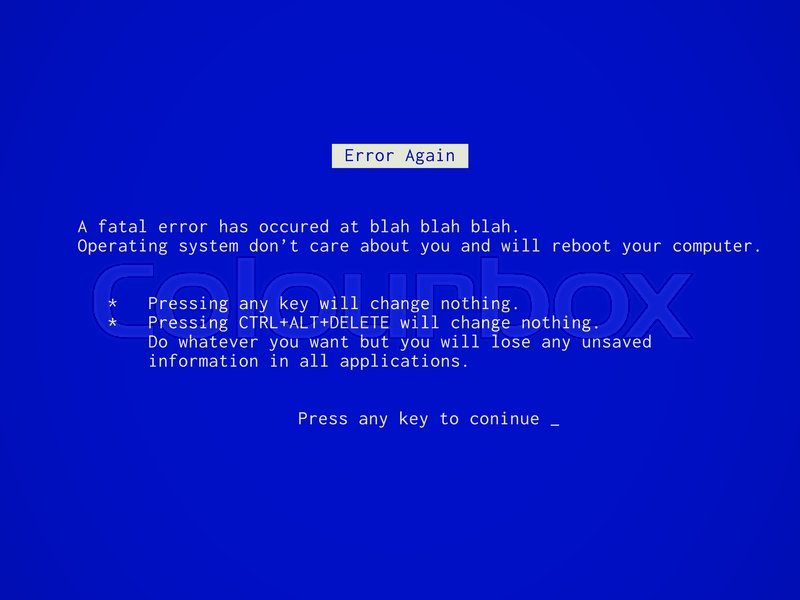
\includegraphics[width=0.8\textwidth,frame]{\CurrentFilePath/ProperScreenshot.png}
\caption{Snippet of the \texttt{runZonedGuarded} method}
\label{figure:code_exception}
\end{figure}

\begin{figure}[H]
\centering
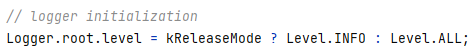
\includegraphics[width=0.8\textwidth,frame]{\CurrentFilePath/code_enabled.png}
\caption{Snippet of the code for setting log level}
\label{figure:code_enabled}
\end{figure}

The aforementioned code snippets can be observed during runtime using the Logcat tool. 
The following screenshot (\cref{figure:logcat}) shows Logcat output during the authentication.

\begin{figure}[H]
\centering
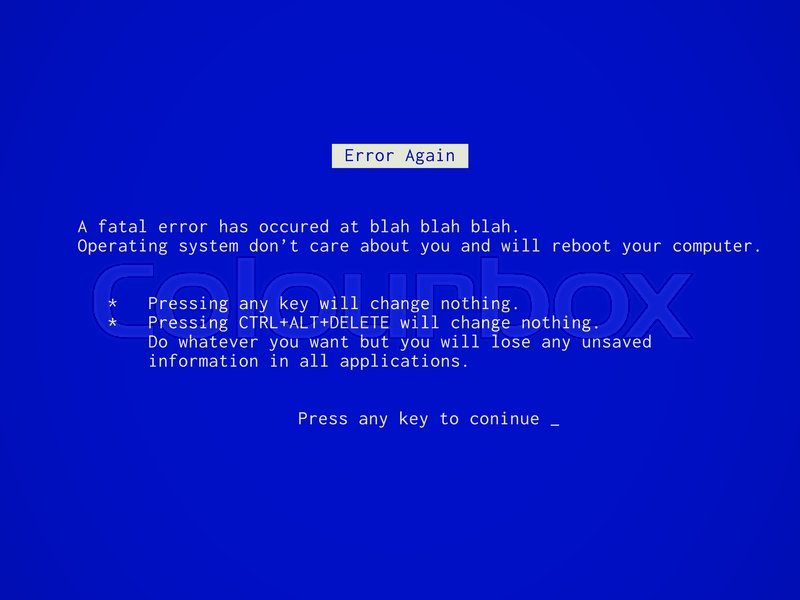
\includegraphics[width=1\textwidth,frame]{\CurrentFilePath/ProperScreenshot.png}
\caption{Logcat output with set filter}
\label{figure:logcat}
\end{figure}

%-<Repeatability>
%-------------------------------------------
%	Countermeasures                        |
%-------------------------------------------



\subsection*{Countermeasures}

It is recommended not to enable logging in the production build or to remove sensitive information from logging, such as JWT and exception stack trace.

%-<Countermeasures>
%-------------------------------------------
%	References - pulls bib entries         |
%-------------------------------------------



\subsection*{References}

This finding references the following information sources:

\begin{itemize}
	\item \href{https://www.first.org/cvss/calculator/3.1#CVSS:3.1/AV:L/AC:L/PR:N/UI:N/S:U/C:L/I:N/A:N}{CVSS 4.0}
	\item \bibentry{CWE-532}
\end{itemize}

%-<References>




